%\documentclass[12pt, a4paper]{book}


%\begin{document}

\chapter{Background}
\label{chap:background}

This chapter includes the background research that founded this bachelor thesis. It is divided into 5 main categories: The Human Personality, The Entrepreneurial Personality, Prediction of the Entrepreneurial Personality, Datasets and lastly, Applications of a Data Benchmark that serves as a high-level introduction to this research.

\section{The Human Personality}
A personality refers to the unique set of individual traits, behaviors, attitudes, and characteristics that distinguish one person from another \cite{kerz2022pushing}. It encompasses the way a person thinks, feels, and behaves across various situations and contexts . Personality is believed to be relatively stable over time but can also be influenced by environmental factors \cite{liao2024open}, experiences, and personal development. Psychologists often study personality to understand how it shapes an individual's thoughts, emotions, motivations, and interactions with others. Personality is closely linked to a broad spectrum of human actions and circumstances, including shopping habits, well-being, social connections, and potentially criminal activities.

The fundamental principle of personality psychology is that stable individual traits lead to consistent behavioral patterns that people tend to show, regardless of the circumstances \cite{vinciarelli2014survey}. Trait models in psychology are constructed based on how people perceive similarities and connections between descriptive words they use to characterize themselves and others. Despite the abundance and diversity of these terms, they generally are reduced  to only a few major dimensions  \cite{vinciarelli2014survey}. 

There are several personality models used in predicting personality, such as Big Five Personality, MBTI (Myers-Briggs Type Indicator) or DISC (Dominance Influence Steadiness Conscientiousness). However, after some considerations and literature review process, Big Five Personality is the most popular and precise in telling someone’s personality traits \cite{kerz2022pushing}, \cite{tandera2017personality}. The model describes human personality by five traits/factors, popularly referred to as the Big Five or OCEAN: Openness to experience, Conscientiousness, Extraversion, Agreeableness, and Neuroticism. These traits are today's dominant paradigm in personality research, and one of the most influential models in all of psychology \cite{mccrae2009five}.

%\footnotetext{Normally named Neuroticism, but we will use the inverse stability throughout the paper to ensure consistently positive factor names.}

The Big Five traits are as follows \cite{bacsaran2021neural}, \cite{antoncic2015big}:\begin{enumerate}
\item \textit{Openness to Experience:}\\
Individuals high in openness tend to have broad interests and are often imaginative, creative, and intellectually curious, and may be more receptive to change. However, they may also be prone to overthinking, indecision, and distraction.

\item \textit{Conscientiousness:}\\
Conscientious individuals are characterized by their strong sense of responsibility, self-discipline, and reliability, and also tend to be organized, and detail-oriented. Though, they may be perceived as rigid, perfectionist, and overly cautious.

\item \textit{Extraversion:}\\
Extraverts are sociable, outgoing individuals and derive energy from interacting with others. They tend to be assertive, and often taking on leadership roles \cite{vinciarelli2014survey}. However, they may also experience struggle with introspection, and be prone to risk-taking behaviors.

\item \textit{Agreeableness:}\\
Agreeable individuals are compassionate, empathetic, and cooperative. They tend to be trusting, forgiving and considerate of others' feelings and needs. However, they may also be vulnerable to exploitation, overly trusting.

\item \textit{Neuroticism:}\\
Neuroticism reflects the tendency to experience negative emotions such as anxiety, depression, and moodiness \cite{vinciarelli2014survey}. Individuals high in neuroticism may be prone to worry, and emotional volatility, struggling with feelings of insecurity, self-doubt, and fear of failure.
\end{enumerate}

\section{The Entrepreneurial Personality}
Moving on to a more specific type of personalities that is the focus of this study, which is the entrepreneurial personality. The term "entrepreneur" originates from the French word "entreprendre" and the German word "unternehmen," both of which convey the concept of "undertaking." As per the Webster dictionary, an "entrepreneur" is someone who organizes, manages, and takes on risks of a business or enterprise \cite{singh2013entrepreneurs}. Enterprising behaviour plays an important role in the modern economy which is characterized by instability and rapid change, obliging people and organizations to be in a process of constant innovation \cite{postigo2021general}.

A person may be enterprising at the personal level (personal entrepreneur), which involves demonstrating a strong sense of control and the ability to manage difficult situations and steer their own life \cite{frese20014}. There are two enterprising personalities we can mention, The intra-entrepreneurs and the extra-entrepreneurs. The intra-entrepreneur refers to people who produce changes and innovation within their positions in a company, adding something creative in their projects that are already in progress \cite{mumford2020intrapreneurship}. The extra-entrepreneur is a person whose goal is the development of new external projects and businesses creation \cite{postigo2021general}. The focus of this thesis will be the extra-entrepreneur, or as known as the "general entrepreneur", a person who chooses to work for themselves, not for others.

Additionally, as there are well known standardized traits that measures the different dimensions of a personality, there are specific traits that provides a more precise description of how entrepreneurs and non-entrepreneurs differ in specific behavioral dimensions \cite{postigo2021general}. These traits are measured using the Measure of Entrepreneurial Tendencies and Abilities (META), which demonstrated that there is a stronger evidence of predictive accuracy with these traits than the Big Five personality traits. META is a state-of-the-art psychometric test that identifies entrepreneurial potential in order to help businesses nurture and retain their entrepreneurial talent. It assesses four aspects of entrepreneurial personality, namely, entrepreneurial awareness, entrepreneurial creativity, opportunism, and vision  \cite{ahmetoglu2011eq}.

Furthermore, after the development of the META, it was discovered that this measuring instrument has focused on a specific trait in an entrepreneur's personality, so there are no comprehensive, exhaustive, systematic analyses of entrepreneurial personality. Then, new eight dimensions of entrepreneurial personality, for young people and adolescents was developed to include all different aspects \cite{suarez2014screening}. The eight specific traits of an entrepreneurial personality are: 
\begin{enumerate}
\item \textit{Self-efficacy:} 
It refers to a person's ability to organize and carry out actions effectively, and their persistence when encountering obstacles.
\item \textit{Autonomy:}
It refers to the motivation for entrepreneurial creation to achieve a certain individual freedom.
\item \textit{Innovativeness:}
It is the will and interest in finding new ways to do usual daily tasks.
\item \textit{Internal locus of control:}
It is about taking responsibility and attributing the consequences of one's actions to their causes.
\item \textit{Achievement motivation:}
It is the desire to achieve standards of excellence.
\item \textit{Optimism:}
It refers to the beliefs a person has about good things happening more than bad things in their life.
\item \textit{Stress tolerance:}
It can be defined as the resistance to perceiving environmental stimuli as stressors due to the appropriate coping strategies.
\item \textit{Risk-taking:}
It is people's tendency and will to assume certain levels of risk or change to achieve an objective.
\end{enumerate}

Figure 2.1 demonstrates the Big Five Personalities and how can we relate them to the eight specific entrepreneurial traits. As each trait of the Big Five traits can be an umbrella for multiple specific traits. 

\begin{figure}[H]
\centering
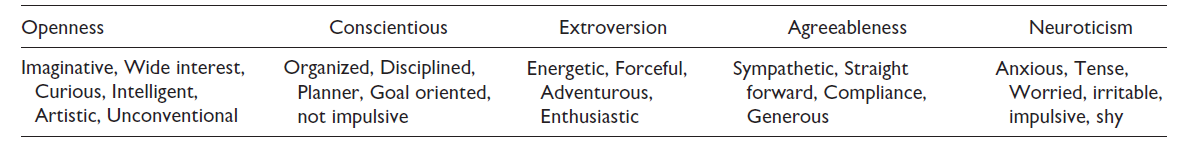
\includegraphics[width=17cm]{Figure1}
\caption{Big Five Personality Traits}
\end{figure}

\section{Prediction of the Entrepreneurial Personality}
In recent years, there has been a significant evolution in how we approach the analysis and prediction of individuals' personalities. Traditional methods heavily relied on standardized questionnaires and self-report measures. Questionnaires where people rate their own behavior with Likert scales are the instrument most commonly adopted for such a purpose \cite{vinciarelli2014survey}. The most popular questionnaires for predicting the general personality traits include the NEO-Personality-Inventory Revised (NEO-PI-R, 240 items), the NEO Five Factor Inventory (NEO-FFI, 60 items), and the Big-Five Inventory (BFI, 44 items). Short questionnaires (5-10 items), much faster to fill, were built by retaining only those items that best correlate with the results of the full instruments \cite{vinciarelli2014survey}.

Further, for the eight specific entrepreneurial personality traits, the Battery for the assessment of the enterprising personality (BEPE) was developed. The items making up the battery follow a Likert-type format with five answer categories (1 totally disagree, 5 totally agree), in line with established psychometric literature which indicates that between four and six answer categories produce better psychometric indicators \cite{cuesta2018assessment}. The main limitation of self-assessments is that the subjects might tend to bias the ratings towards socially desirable characteristics, especially when the assessment can have negative consequences \cite{vinciarelli2014survey}. 

However, with the rise of technological advancements and social media platforms, there has been a notable shift towards extracting more data from naturalistic data sources. Several works investigate the interplay between personality and computing by measuring the link between traits and use of technology. Online social networks like Twitter, Google+ and Facebook contain much information that can potentially reveal many traits, preferences and opinions of the profile owner. This resulted in research on personal analytic – automatically inferring such latent author attributes in social media \cite{el2022deep}, \cite{tandera2017personality}, \cite{volkova2015inferring}, \cite{vinciarelli2014survey}.

Given its central importance in capturing the essential aspects of human life, increasing attention is being paid to the development of models that can use behavioral data to automatically predict personality. Affective computing focuses on introduces novel techniques that develop and apply affective reasoning tools for personality prediction in multiple modalities and different languages \cite{el2022deep}. They infer personality traits from audio, static image, video, or audio visual clip recorded from various scenarios, such as dyadic dialogue, self-evaluating surveys and self-interviews \cite{liao2024open}. Data obtained from verbal behavior is one of the key types of such data. Even in the early years of psychology, a person's use of language was seen as a distillation of his or her underlying drives, emotions, and thought patterns \cite{kerz2022pushing}. 

With the aid of machine learning models, researchers and practitioners can extract valuable insights from unstructured textual data, such as emails, social media posts, and online forums. By analyzing language patterns, word choices, and linguistic styles, these models can discern underlying personality traits with a higher degree of accuracy than traditional questionnaires \cite{kerz2022pushing}, \cite{volkova2015inferring}, \cite{akrami2019automatic}. These measurements capture the within-text distributions of scores for a given psycholinguistic feature, referred as "text contours". There are four main groups for these features \cite{kerz2022pushing}, \cite{tandera2017personality}, \cite{vinciarelli2014survey}, \cite{el2022deep}:
\begin{enumerate}
\item \textit{Features of morpho-syntactic complexity:}
This group includes surface features such as the average length of clauses and sentences, the features of the type and frequency of embeddings like the number of dependent clauses or the verb phrases, and finally the frequency of particular structure types.

\item \textit{Features of lexical richness, diversity and sophisticated:}
This group includes the lexical density features, like the ratio of lexical words to the total number of words in a text. Also, it includes the lexical variation such as the vocabulary used, the lexical sophistication, for the unusual or advanced words in a text, the psycholinguistic norms of words, and lastly, how much people know this word.

\item \textit{Readability features:}
This group combines a word familiarity variable from a prespecified vocabulary resource, along with a syntactic variable, such as average sentence length.

\item \textit{Lexicon features:}
This last group is derived from a total of ten lexicons that have been successfully used in personality detection, emotion recognition and sentiment analysis research, such as The Affective Norms for English Words (ANEW), DepecheMood++, The Linguistic Inquiry Word Count (LIWC) dictionary, etc \cite{pennebaker1999linguistic}. 
\end{enumerate}

The aim of this thesis is to gather all the textual characteristics of texts entrepreneurs write and post on their different platforms, and to distinguish if all entrepreneurs write in a unique way, more sophisticated one than non-entrepreneurs.

\section{Datasets}
In order to predict the entrepreneurial personality, and achieve high accuracy in whatever deep learning model used, there has to be a standardized benchmark data to train these models with. Depending on this dataset, the accuracy of the prediction can change and achieving a state-of-the-art models. In this part, we will discover the process of engineering such a dataset, through studying how different benchmark data used to train models to predict the human personality like well-known datasets: The Stream-of-consciousness Essays Database \cite{pennebaker1999linguistic}, myPersonality \cite{kosinski2015facebook}, and built datasets for specific researches.

Starting with the Essays Dataset \cite{pennebaker1999linguistic}, the database encompasses a diverse range of texts, including novels, short stories, and essays, from various literary periods and cultural contexts. On their first Phase, they defined all the reliability of the language use like the text analysis procedures using the LIWC program, which includes words and categories like emotion category and a sub-category whether it is a negative or positive emotion. Also, they specified the language composition, such as the total number of words, the number of words per sentence, and the number of questions, percentage of unique words, etc. Secondly, they gathered 3 samples of essays from three different sources. The first sample was in a form of daily writings from 15 residential patients in a substance abuse and addiction treatment center in England. The second sample was in a form of daily class assignments by Taos summer school students in New Mexico. The last sample was a group of published abstracts by 40 prominent social psychologists. Each writing sample for each participant was transcribed into a computer text file and analyzed with LIWC program, and the result is described in Figure 2.1.\\
For their second phase, the 1203 essays were from original psychology student samples as assignments of their fall semester in university. These students also completed occasional questionnaires such as the Five Factor Inventory, these answers were used as a labeling for all the essays. Figure 2.2 shows the correlations between the language dimensions and the Five Factor answers. This dataset is considered as a benchmark data, used till this day to train models to predict personality traits.

\begin{figure}[H]
\centering
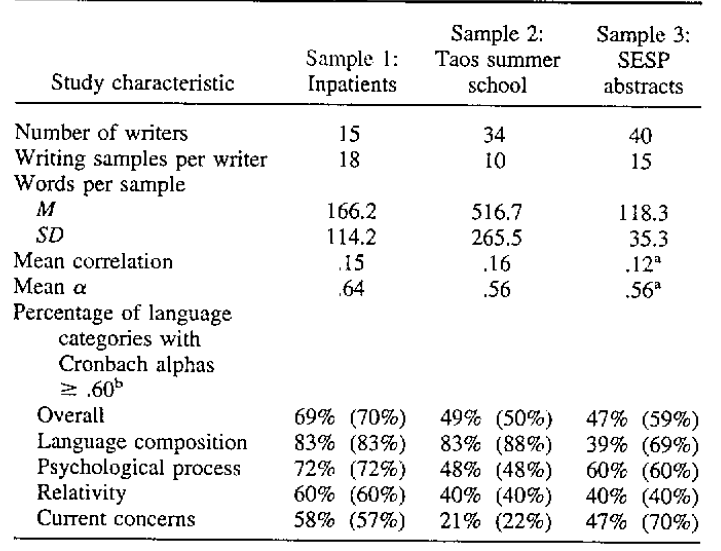
\includegraphics[width=8cm]{Table1}
\caption{Summary of Reliability Studies}
\end{figure}

\begin{figure}[H]
\centering
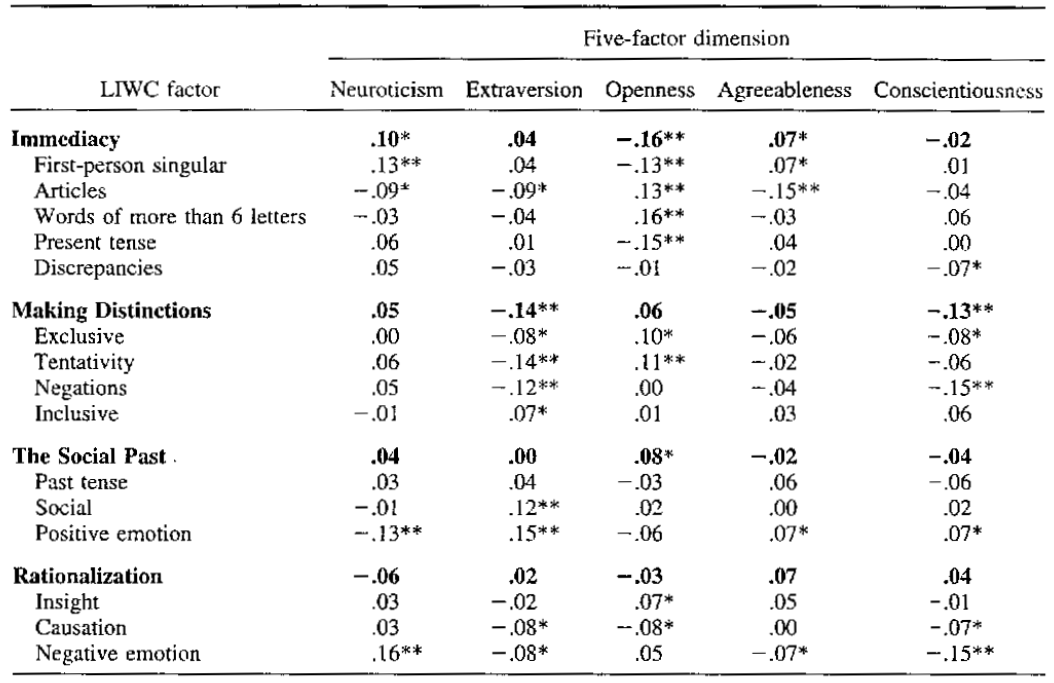
\includegraphics[width=10cm]{Table2}
\caption{LIWC factors and Simple Correlations With Five-Factor Scores}
\end{figure}
Furthermore with the myPersonality Database \cite{kosinski2015facebook}, the paper discusses the distinct opportunities and challenges offered by Facebook to researches. It permitted users to complete genuine psychometric assessments and receive immediate results. Alongside test data, approximately 40\% of participants also chose to share information from their Facebook profiles, resulting in one of the largest social science research databases in history. Respondents came from various age groups, backgrounds and cultures. The Database myPersonality offered a 360-degree
assessment feature, encouraging users to invite their friends to judge their personality.  This resulted in a database of cross-ratings,4 while also helping to increase the virality of the application; those who were invited to rate their friends often proceeded to take a test themselves. A sample of how the dataset was build is shown in Figure 2.3. The app remained operational until 2012, amassing data from over 6 million volunteers in 4 years. In April 2018, the researchers decided to stop sharing the data with other scholars. 
\begin{figure}[H]
\centering
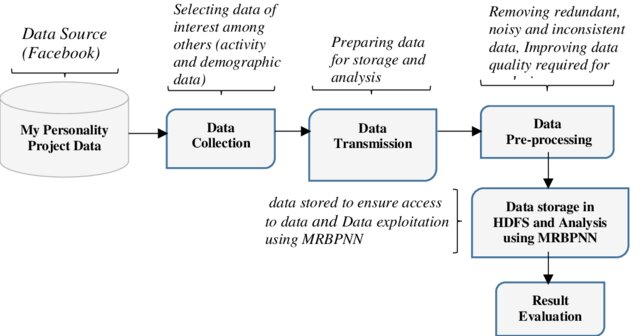
\includegraphics[width=10cm]{Figure3}
\caption{Process to engineering a dataset}
\end{figure}
Moving on to a database that was built to predict the Big Five personality traits on a scale from -3 to 3, rather than a binary classification \cite{akrami2019automatic}. The researchers required training data, to represent the whole data range for each trait in Swedish language. They proceeded by retrieving data from four different Swedish discussion forums and news sites with authors of different personalities. Web spiders were used to download the texts, and they were 70 million texts in total, but they ended up with only 39,370 texts that could be annotated. The texts were annotated by 18 psychology students, each annotated a random text with a specific trait from the Big Five personality traits on a discrete integer interval from -3 to 3 as shown in Figure 2.4. Due to the small number of annotators and the big amount of texts, each text approximately was annotated once. So, it was decided that a smaller subset of the large database would be taken and annotated furthermore, which resulted in a smaller dataset with 2,774 texts, with on average 4.5 annotations each as shown in Figure 2.5.

\begin{figure}[H]
\centering
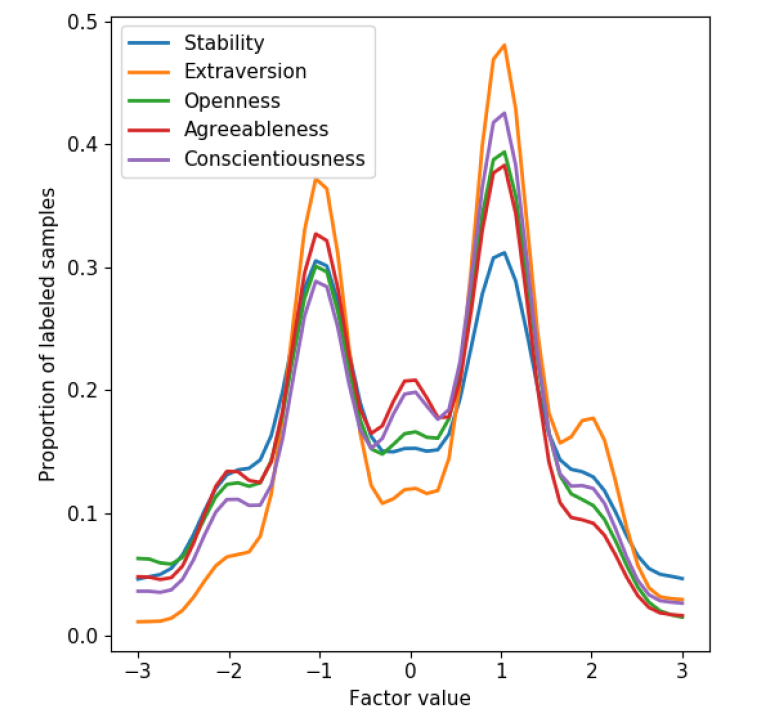
\includegraphics[width=7cm]{Figure4}
\caption{Distribution of labeled samples for each of the factors of the large dataset.}
\end{figure}

\begin{figure}[H]
\centering
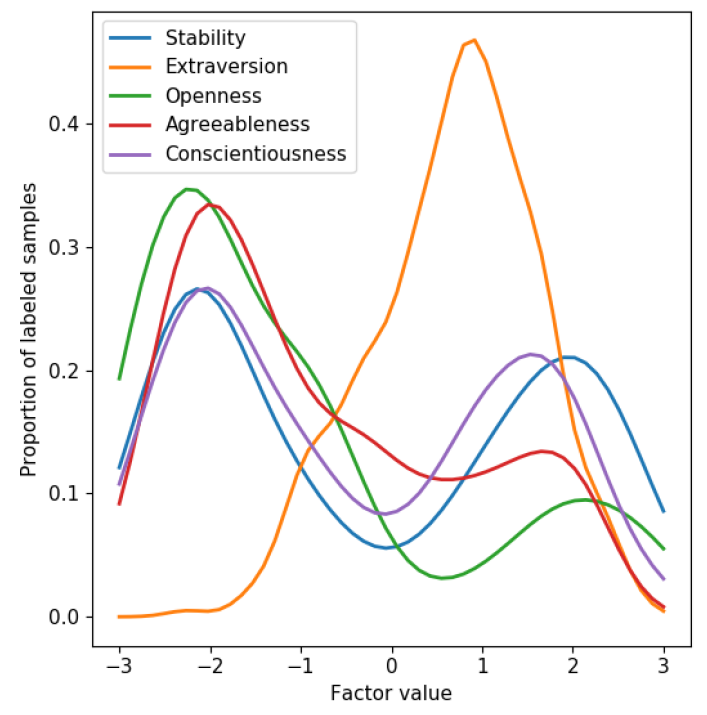
\includegraphics[width=7cm]{Figure5}
\caption{Distribution of labeled samples for each of the factors of the small dataset.}
\end{figure}

For feature extraction, ther used Term Frequency-Inverse Document Frequency (TF-IDF) to construct features from labeled data. It was used on word and character level with bi-gram for words and quad-grams for characters. Several regression models were tested, and they used ULMFiT as their NLP. The performance of the models was evaluated with 5-fold cross validation test, as well as a binary classification test, and they did test their model on wild data like Cover Letters Dataset and Self-Descriptions Dataset. At the end, they were able to create models with reasonable performance, with accuracy in-line with the state-of-the-art models. And, it was found that using a smaller amount of high-quality training data with multi-annotator assessments resulted in models that outperformed models based on a large amount of solo-annotated data. Their results showed that extracting personality traits from a text remained a challenge.

\section{Applications of The Benchmark Data}
Imagine yourself as an recruiter standing in your company's booth in a career fair, meeting all the undergraduates and the graduates, and you are searching to recruit someone for a position with a high leadership skills, innovative, independent, and most importantly a risk taker. You have a new tool at the reach of your hands, to just let the student write a paragraph about himself, and from this paragraph, you will be provided with a direct response if this person has the potential of being an entrepreneur or not, and a detailed explanation on whether or not he should proceed to the next recruitment phase.

Analyzing a simple textual post or comment to predict of the author has the potential to be an entrepreneur or not, or he is already an entrepreneur and owns a business, would be a great asset for companies, for a country's economy and for this person's own self-development. Predicting the entrepreneurial personality can have several application and benefits. Firstly, in the realm of recruitment and selection, companies can harness personality assessments to pinpoint individuals possessing traits conducive to entrepreneurship. By identifying candidates with characteristics such as risk-taking propensity, creativity, and proactiveness, organizations can assemble teams better equipped to innovate and drive business growth \cite{el2022deep}. 

On an individual level, personality assessments provide valuable insights into one's entrepreneurial strengths, weaknesses, and areas for development. By understanding their entrepreneurial personality profile, individuals can focus on honing relevant skills and attributes to enhance their chances of success in entrepreneurial endeavors. Also, it can help social network users to understand how others may perceive them based on how they communicate in social media, in addition to its evident applications in online sales and marketing, targeted advertising, large scale polling and healthcare analytics \cite{volkova2015inferring}.

Similarly, organizations providing business incubation and support services to start-ups can utilize personality assessments to tailor their assistance to the specific needs of entrepreneurs. By understanding the personality profiles of their clients, these organizations can offer targeted mentoring, resources, and networking opportunities to support the start-ups' entrepreneurial journey and maximize their chances of success \cite{antoncic2015big}.

Lastly, at a broader level, policymakers and economic development agencies can leverage personality analysis to understand the entrepreneurial culture within a region or community. By identifying individuals with entrepreneurial potential and providing support and resources to foster their endeavors, policymakers can cultivate a vibrant entrepreneurial ecosystem conducive to economic development and job creation. Policy-makers might like to consider promoting and enhancing entrepreneurship predictive personality factors (particularly openness) early on in the education system among children, teens and students who have the potential to become entrepreneurs \cite{antoncic2015big}.

\bibliographystyle{ieeetr}
\bibliography{citations.bib}

%\end{document}